% $Header: /cvsroot/latex-beamer/latex-beamer/examples/beamerexample5.tex,v 1.22 2004/10/08 14:02:33 tantau Exp $

\documentclass[11pt]{beamer}

\usetheme{Darmstadt}

\usepackage{times}
\usefonttheme{structurebold}

%\usepackage[english]{babel}
\usepackage[portuges]{babel}
\usepackage{pgf,pgfarrows,pgfnodes,pgfautomata,pgfheaps}
\usepackage{amsmath,amssymb}
\usepackage[utf8]{inputenc}
\usepackage[T1]{fontenc}
\usepackage{graphicx}

\setbeamercovered{dynamic}

\newcommand{\Lang}[1]{\operatorname{\text{\textsc{#1}}}}

\newcommand{\Class}[1]{\operatorname{\mathchoice
  {\text{\sf \small #1}}
  {\text{\sf \small #1}}
  {\text{\sf #1}}
  {\text{\sf #1}}}}

\newcommand{\NumSAT}      {\text{\small\#SAT}}
\newcommand{\NumA}        {\#_{\!A}}

\newcommand{\barA}        {\,\bar{\!A}}
\def\bbar{{\mathchar'26\mkern-9mu b}}
\def\dbar{{\mathchar'26\mkern-12mu d}}
\newcommand{\Nat}{\mathbb{N}}
\newcommand{\Set}[1]{\{#1\}}

\pgfdeclaremask{tu}{beamer-tu-logo-mask}
\pgfdeclaremask{computer}{beamer-computer-mask}
\pgfdeclareimage[interpolate=true,mask=computer,height=2cm]{computerimage}{beamer-computer}
\pgfdeclareimage[interpolate=true,mask=computer,height=2cm]{computerworkingimage}{beamer-computerred}
\pgfdeclareimage[mask=tu,height=.5cm]{logo}{logounesp}

\logo{\pgfuseimage{logo}}

\title{Forças Termodinâmicas}
\author{Ney Lemke}
\institute[IBB-UNESP]{%
    Biofísica e Farmacologia}
\date{ \today}                                

\colorlet{redshaded}{red!25!bg}
\colorlet{shaded}{black!25!bg}
\colorlet{shadedshaded}{black!10!bg}
\colorlet{blackshaded}{black!40!bg}

\colorlet{darkred}{red!80!black}
\colorlet{darkblue}{blue!80!black}
\colorlet{darkgreen}{green!80!black}

\def\radius{0.96cm}
\def\innerradius{0.85cm}

\def\softness{0.4}
\definecolor{softred}{rgb}{1,\softness,\softness}
\definecolor{softgreen}{rgb}{\softness,1,\softness}
\definecolor{softblue}{rgb}{\softness,\softness,1}

\definecolor{softrg}{rgb}{1,1,\softness}
\definecolor{softrb}{rgb}{1,\softness,1}
\definecolor{softgb}{rgb}{\softness,1,1}

\AtBeginSection[]{\frame{\frametitle{Outline}\tableofcontents[current]}}

\begin{document}



\frame{\titlepage}



\section{Introdução}
\frame{\frametitle{Sistemas Termodinâmicos}
  \begin{itemize}
  \item Sistema formado por uma grande quantidade de átomos.
  \item Ausência de correntes.
  \item Estacionário.
  \item Comportamento independente da história.
  \end{itemize}

}

\frame{\frametitle{Definições}
  \begin{description}
  \item[Sistema Aberto] Um sistema aberto pode trocar energia, volume
    e matéria com o ambiente.
  \item[Sistema Fechado] Troca energia mas não troca matéria.
  \item[Sistema Isolado] Não troca nem energia nem matéria.
  \item[Fronteira Adiabática] Impede a troca de calor entre o sistema e o meio.
\end{description}
}

\frame{\frametitle{Definições}
  \begin{description}
  \item[Fase] É uma parte homogênea de um sistema físico.
  \item[Sistema Simples] Sistema composto por uma única fase.
  \end{description}
}

\frame{\frametitle{Propriedades Extensivas}
  \begin{description}
  \item[Extensiva] Uma propriedade $P$ é dita extensiva se ela for a soma das 
propriedades $P_i$ de seus subsistemas.
\item[Intensiva] Uma propriedade é dita intensiva se for obtida pela razão 
de uma propriedade extensiva e o número de moléculas de um sistema.
\item[Energia Interna] A energia interna $U$ de um sistema é extensiva. Para 
um sistema composto por $N$ partículas a energia é a soma das energias de cada uma das partículas.:

$$U=\sum_i^t N_i\epsilon_i$$

$N_i$ representa o número de partículas que possuem a energia $\epsilon_i$.
  \end{description}
}

\section{Equações Fundamentais}

\frame{\frametitle{Equação Termodinâmica Fundamental}

$$S=S(U,V,\mathbf{N})$$

ou 

$$U=U(S,V,\mathbf{N})$$

}


\frame{\frametitle{Forças Termodinâmicas}
%\left( \frac{\partial }{\partial }\right)_{}d

$$dS=\left( \frac{\partial S}{\partial U}\right)_{V,N}dU+
\left( \frac{\partial S}{\partial V}\right)_{U,V}dV+
\sum_{j=1}^N\left( \frac{\partial S}{\partial N_j}\right)_{U,V,N_{i\neq j}}dN_j$$

$$dU=\left( \frac{\partial U}{\partial S}\right)_{V,N}dS+
\left( \frac{\partial U}{\partial V}\right)_{S,N}dV+
\sum_{j=1}^N\left( \frac{\partial U}{\partial N_j}\right)_{S,V,N_{i\neq j}}dN_j$$


}


\frame{\frametitle{Forças Termodinâmicas}
  \begin{description}
  \item[Temperatura]
$$T=\left( \frac{\partial  U}{\partial S}\right)_{V,\mathbf{N}}$$
  \item[Pressão]
$$p=-\left( \frac{\partial U}{\partial V}\right)_{S,\mathbf{N}} $$
  \item[Potencial Químico] 
$$\mu_j=\left( \frac{\partial U}{\partial N_j}\right) $$
  \end{description}
}

\frame{\frametitle{Forças Termodinâmicas}
$$dU=TdS-pdV+\sum_j \mu_j dN_j$$

$$dS=\left(\frac{1}{T}\right) dU+\left(\frac{p}{T} \right)dV-\sum_j\left(  \frac{\mu_j}{T} \right)dN_j$$
}

\frame{\frametitle{Foras Termodinmicas}
$$\left(\frac{1}{T}\right)=\left( \frac{\partial S}{\partial U}\right)_{V,N} \quad
\left( \frac{p}{T} \right)=\left( \frac{\partial S}{\partial V}\right)_{U,N}$$

$$
\left( \frac{\mu_j}{T}\right)_{S,V,N_{i\neq j}}=\left(\frac{\partial S}{\partial N_j}\right)_{U,V,N_{i\neq j}}$$
}

\frame{\frametitle{Gás Ideal}
Considere um sistema formado por $N$ partículas em uma rede linear de tamanho $M$.

$$\frac{S}{k}=\ln W(N,M)=\ln \left( \frac{M!}{N!(N-M)!}\right)$$

$$\frac{p}{T}=\left( \frac{\partial S}{\partial V}\right)_{U,N}$$

$$\left( \frac{\partial S}{\partial V}\right)_{U,N}=
\left( \frac{\partial S}{\partial M}\right)_{U,N}\left( \frac{\partial M}{\partial V}\right)_{U,N}=\left( \frac{\partial S}{\partial M}\right)_{U,N}\left( \frac{M}{V}\right)$$

}

\frame{\frametitle{Gas Ideal}

$$\frac{S}{k}=-N\ln \left( \frac{M}{N} \right)-(M-N)\ln \left( \frac{M-N}{M}\right)$$


$$\left( \frac{\partial S}{\partial M}\right)_N=-k\ln \left( 1-\frac{N}{M} \right)$$

$$p=-kT\left(\frac{M}{N}\right)\ln \left( 1-\frac{N}{M} \right)$$

$$p=\left( -\frac{MkT}{V}\right) \left( -\frac{N}{M}\right)\left(1+\frac{1}{2}\left(\frac{N}{M}\right)+\ldots \right)\sim \frac{NkT}{V}$$
}

\frame{\frametitle{Grandezas Extensivas e Intensivas}

  \begin{description}
  \item[Extensivas] $U$, $V$ $N$ e $S$
  \item[Intensivas] $p$, $T$ $\mu$
  \end{description}

}

\frame{\frametitle{Funções Homogêneas}
$$f(\lambda x_1,\lambda x_2,\ldots , \lambda x_M)=\lambda f(x_1,x_2,\ldots ,x_M)$$

$$\frac{df(\lambda x_1,\lambda x_2,\ldots , \lambda x_M)}{d\lambda}=f(x_1,\ldots,x_M )
=\sum_i \left( \frac{\partial f}{\partial(\lambda x_i)} \right) 
\left(\frac{\partial \lambda  x_i}{\partial \lambda} \right)
$$

$$f=\sum_i x_i \left( \frac{\partial f}{\partial(\lambda x_i)} \right) $$

Se $\lambda=1$, temos que:

$$f=\sum_i x_i \left( \frac{\partial f}{\partial x_i} \right) $$
}

\frame{\frametitle{Funções Homogêneas}

$$U=TS-pV+\sum_i \mu_i N_i$$

}
\section{Forças Termodinâmicas}


\frame{\frametitle{Temperatura e Calor}
Considere dois sistemas $A$ e $B$ separados por uma parede 
adiabática. 

A Entropia e a Energia Interna do sistema composto é:

$$S=S_A+S_B \quad U=U_A+U_B=\mbox{cte}$$ 

$$dS=dS_A+dS_B=\left( \frac{\partial S_A}{\partial U_A}\right)_{V,N}dU_A+\left( \frac{\partial S_B}{\partial U_B}\right)_{V,N}dU_B=0$$

$$dU=0\quad dU_A=-dU_B$$
}

 \frame{\frametitle{Temperatura e Calor}
 $$dS=\left[ \left( \frac{\partial S_A}{\partial U_A}\right)_{V,N}-\left( \frac{\partial S_B}{\partial U_B}\right)_{V,N} \right]dU_A=0$$

$$ \left( \frac{\partial S_A}{\partial U_A}\right)_{V,N}=
    \left( \frac{\partial S_B}{\partial U_B}\right)_{V,N}$$



 $$\frac{1}{T_A}=\frac{1}{T_B}\quad T_A=T_B$$


}

\frame{\frametitle{Direo da Transmisso de Calor}
$$dS=\left( \frac{1}{T_A}-\frac{1}{T_B} \right) dU_A\geq 0$$

Se $dU_A>0$ então $T_B>T_A$. Ou seja se o objeto $A$ ganha energia sua temperatura é menor. 
O calor flui para o corpo mais frio. 
}

\frame{\frametitle{Interpretao da Temperatura}
  \begin{center}
    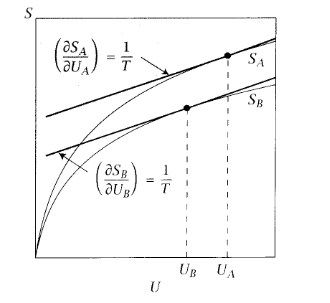
\includegraphics[scale=0.5]{temp}
  \end{center}
Analogia Financeira: Dinheiro  Energia e Entropia  funo Utilidade.
}

\frame{\frametitle{Presso e Volume}
 \begin{center}
    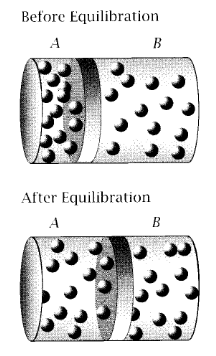
\includegraphics[scale=0.3]{pressao}
  \end{center}

$$dV_A=-dV_B$$
$$T_A=T_B$$

}

 \frame{\frametitle{Presso e Volume}

 $$dS=dS_A+dS_B$$
$$=\left( \frac{\partial S_A}{\partial V_A}\right)_{U,N}dV_A+\left( \frac{\partial S_B}{\partial V_B}\right)_{U,N}dV_B+$$
$$\left( \frac{\partial S_A}{\partial U_A}\right)_{V,N}dU_A+$$
$$
\left( \frac{\partial S_B}{\partial U_B}\right)_{V,N}dU_B=0=0$$

$$dS=\left[\left( \frac{\partial S_A}{\partial V_A}\right)_{U,N}+\left( \frac{\partial S_B}{\partial V_B}\right)_{U,N}\right]dV_A=0$$

$$\left[ \frac{p_A}{T}-\frac{p_B}{T} \right]=0 \quad p_A=p_B$$

}


 \frame{\frametitle{Presso e Volume}
$$dS=\left[ \frac{p_A}{T}-\frac{p_B}{T} \right]dV_A\geq 0$$
Se $dV_A>0$ ento $p_A>p_B$ ou seja se o volume aumenta isto ocorre porque $p_A>p_B$.
}

\frame{\frametitle{Potencial Qumico }
Suponha que eu possua um sistema formado por dois subsistemas separados
por uma membrana permeável. Supomos que a pressão e a Temperatura sejam iguais 
nos dois lados. 

$$dN_A=-dN_B$$

$$dS=\left(\frac{\partial S_A}{\partial N_A} \right)dN_A+\left(\frac{\partial S_B}{\partial N_B} \right)dN_B$$

$$dS=\left(\frac{\mu_a}{T}-\frac{\mu_B}{T}  \right)dN_A=0\quad \mu_A=\mu_B$$

$$dS=\left(\frac{\mu_B}{T}-\frac{\mu_B}{T}  \right)dN_A$$
 }

\section{Processos}


 \frame{\frametitle{Diferenciais Exatos}

Considere uma função $H(x,y)$:

$$dH= \left( \frac{\partial H}{\partial x}\right)_y+
\left( \frac{\partial H}{\partial y}\right)_x$$

Mas considere a situao reversa, considere o diferencial:

$$M(x,y)dx+N(x,y)dy$$

Ser que existe $G$ tal que $dG$ seja este diferencial?
}

\frame{\frametitle{Diferenciais Exatos}
Em geral não. É condição necessária e suficiente para a existência de $G$ que:

$$\left(\frac{\partial M}{\partial y} \right)=\left(\frac{\partial N}{\partial x} \right)$$

Quando um referencial satisfaz essa condição é chamado de diferencial exato. Caso contrário 
é chamado de diferencial inexato e denotado por
$\delta w$  ou $\dbar w$.

}


\frame{\frametitle{Diferenciais Exatos}
Se temos um diferencial exato ento:

$$\oint dG =0$$

Mas

$$\oint \delta G\neq 0$$

}

 \frame{\frametitle{Trabalho}

$$\delta w=-pdV$$

   \begin{description}
   \item[Volume Constante] $w=0$
   \item[Presso Constante] $w=-p\Delta V$
   \item[Temperatura Constante] 
$$w=-NkT\ln \frac{V_B}{V_A}$$
   \end{description}
 }

\frame{\frametitle{Processo Adiabtico}

Neste processo a Entropia no varia.

$dU=\delta W$

Suponha um gs ideal. Neste caso temos que 

$$U=\frac{3}{2} kT \quad pV=NkT$$
}

\frame{\frametitle{Processo Adiabtico}
$$\frac{3}{2} Nk dT=-pdV=-\frac{NkT}{V}dV$$

$$\frac{3}{2} \frac{dT}{T}=-\frac{dV}{V}$$

$$\frac{V_f}{V_i}=\left( \frac{T_i}{T_f}\right)^{3/2}$$
}


\frame{\frametitle{Primeira Lei}

$$dU=\delta q+\delta w$$
}

\frame{\frametitle{Segunda  Lei}
$$dU=TdS-pdV$$

$$dU=\delta q+\delta w=\dbar q-pdV$$

$$Tds=\delta q$$

}

\frame{\frametitle{Ciclo de Carnot}
  \begin{center}
    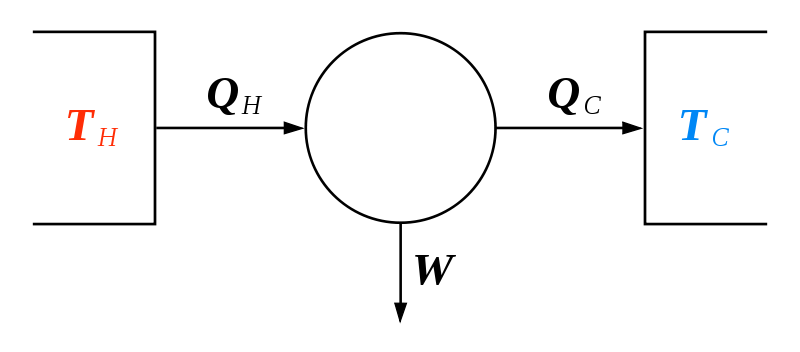
\includegraphics[scale=0.4]{carnot}
  \end{center}

}

\frame{\frametitle{Ciclo de Carnot}
\begin{tabular}{c c}
  \begin{minipage}{0.45\textwidth}
  \begin{itemize}
  \item Expanso Isotrmica
  \item Expanso  Adiabtica
  \item Compresso Isotrmica
  \item Compresso Adiabtica
  \end{itemize}      
    \end{minipage}&

    \begin{minipage}{0.45\textwidth} 
 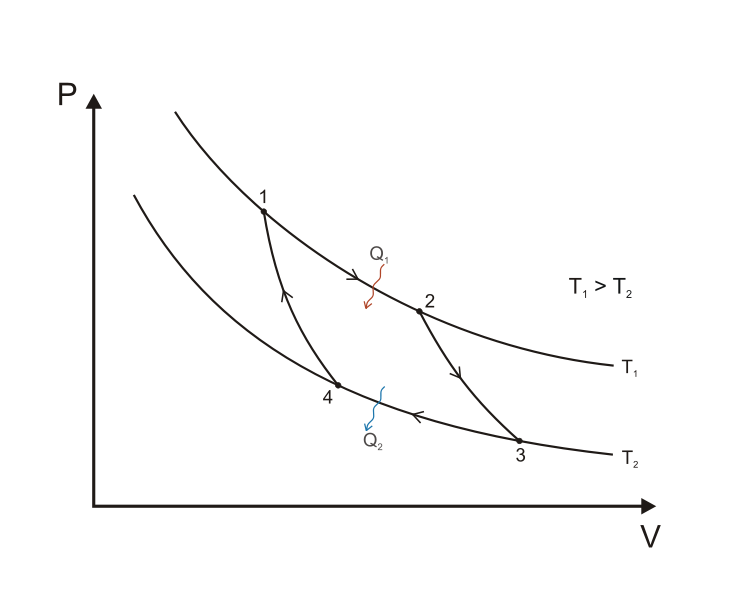
\includegraphics[scale=0.2]{carnot2}
   \end{minipage}
  \end{tabular}
}

\frame{\frametitle{Ciclo de Carnot}
\begin{tabular}{c c}
  \begin{minipage}{0.45\textwidth}
 $$dU=0 \quad \delta q=-\delta w$$
$$W=\oint TdS$$
$$=(T_H-T_C)(S_B-S_A)$$
$$Q_H=T_H (S_B-S_A)$$
$$\eta =\frac{W}{Q_H}=\left( 1- \frac{T_C}{T_H} \right)$$
    \end{minipage}&

    \begin{minipage}{0.45\textwidth} 
 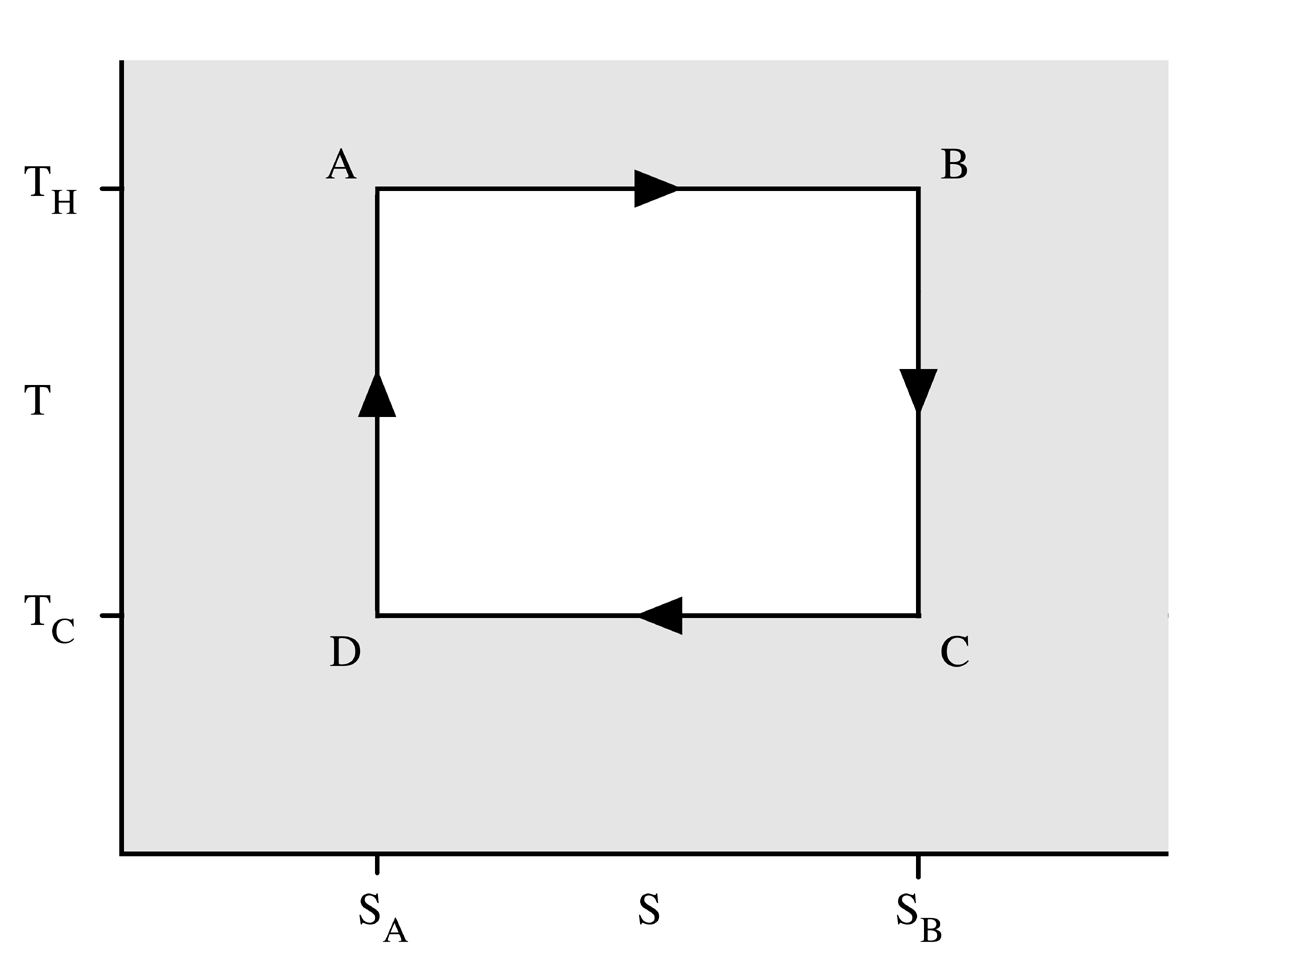
\includegraphics[scale=0.1]{carnot3}
   \end{minipage}
  \end{tabular}
}


\frame{\frametitle{Escala Absoluta de Temperatura}


}
\end{document}
